\documentclass[12pt]{report}
\usepackage[margin=1.0in,a4paper]{geometry}
\usepackage{graphicx}
\usepackage{subfigure}
\usepackage{float}
\usepackage{setspace}
\usepackage{amsmath}
\usepackage{cite}
%opening
%\title{Human microRNAs Exhibit Two Distributions Within and Across Cancer Samples}
%\author{Eric T Dawson}
\singlespace


\begin{document}
\begin{titlepage}
\begin{center}
% \maketitle
 \includegraphics[scale=.2]{/Users/eric/Dropbox/thesis/UTseal.png}
 \vfill
 \Huge \textbf{Human microRNAs exhibit two distributions of expression within and across cancer samples}
 \vfill
\noindent
\begin{minipage}[t]{0.4\textwidth}
\begin{flushleft} \large
\emph{Author:}\\
Eric Thomas Dawson
\end{flushleft}
\end{minipage}%
\begin{minipage}[t]{0.4\textwidth}
\begin{flushright} \large
\emph{Supervisor:} \\
Dr.~Claus O. Wilke
\end{flushright}
\end{minipage}
\vfill
\large May 08, 2015

\large \textit{For completion of the Dean's Scholars Honors Program}
\end{center}
\vfill

\vfill

\end{titlepage}





\section*{Abstract}
It has been previously established that mRNAs exhibit a distinct pattern of two overlapping distributions in expression \cite{Hebenstreit2011}.
We set out to explore whether the same pattern held in microRNAs.
We used RNA-Seq data from The Cancer Genome Atlas to examine the overall profile of microRNA expression data and fit kernel density estimates.
Our results indicate that microRNA expression does fit into two
distributions, but that the characteristics of these distributions are quite different from those of messenger RNAs. These distributions  seem to have differing abilities
to distinguish tumors within and across cancer types. These trends are consistent across the entirety of the TCGA datasets in our analysis.

\section*{Background}
MicroRNAs are a family small non-coding RNA molecules. First discovered in \emph{C. elegans},
they are conserved across nearly all metazoan species \cite{Ambros2004}.
Mature microRNAs are 20-22bp in size and bind to messenger RNAs through partial 
Watson-Crick base pairing in the 3' untranslated region. While canonically thought of as post-transcriptional 
repressors of messenger RNA activity, in recent years several studies have found 
that microRNAs occasionally act as translational activators \cite{Hammond2006, Gartel2008}.

In humans, the number of microRNAs and predicted targets has expanded greatly since their discovery.
The total number of verified microRNAs in humans  stretches well into the 
hundreds \cite{Barbarotto2008}, with predictions for many more \cite{Friedlander2014}. As a single microRNA can target 
many messenger RNAs, the total number of microRNA targets is significantly 
larger than the number of microRNAs.   Lim \emph{et al} showed that misregulation of 
a single microRNA may affect the expression of over one hundred mRNA 
transcripts \cite{Lim2005}. In aggregate, the number of messenger RNAs targeted by 
microRNAs in humans may constitute more than a third of all known protein coding genes
 \cite{Wang2011}.
 
 
With so many targets, microRNAs are essential regulators of many cellular processes \cite{Ambros2004}.  
As microRNAs must be processed by the enzyme Dicer to become active, Dicer 
mutants have a phenotype analogous to complete knockout of microRNA regulation. 
Dicer mutants of many species do not survive or reproduce, indicating that microRNAs are essential both
during and after development \cite{Bushati2007, Sayed2011}. The irregular expression of microRNAs has been 
associated with a variety of diseases from liver disease to schizophrenia \cite{Wang2012, Beveridge2012}.
In addition, microRNA dysregulation has been associated with nearly all common 
cancer types \cite{Calin2006, Sayed2011}
%TODO cite some disease.


MicroRNAs are of particular interest to cancer researchers because of their 
complex roles in regulating cell processes. Several individual microRNAs have been 
associated with specific cancer types \cite{Calin2006, Eun2007, Yan2014}.
Certain cancer types also show specific microRNA signatures, notably pancreatic
and triple-negative breast cancer \cite{Eun2007, Sayed2011}.
A pan-cancer superfamily of microRNAs has been discussed and seems to define
tumors across many different cancer subtypes \cite{Hamilton2013}. Such 
signatures can help cluster similar patients and act as biomarkers that may 
indicate clinical outcome.


% Clustering, Cell type specificity

A major frontier in cancer research at the moment is the use of high-throughput
techniques to stratify patients within cancer types to provide treatment more 
tailored to the individual's pathology. In addition, these algorithms aim
to prevent misdiagnosis of a metastasis as the primary tumor; while this is a rare mistake
it has a profoundly negative effect on patient outcome. Several models for molecular patient stratification
have been introduced. In the past these models used expression data from
microarrays. Modern examples use their own subsets of pan-cancer ``omics'' data
to make inferences about 
the molecular pathology of a tumor. Many also employ new or different clustering 
algorithms to achieve better performance. The two predominant algorithms, 
Network-Based Stratification (NBS) \cite{Hofree2013} and PARADIGM \cite{Vaske2010}
both use protein-protein interaction networks to classify tumors based on 
impacted cellular pathways. NBS uses a patient's predicted set of somatic
mutations while PARADIGM uses DNA, RNA, 
and protein data abstracted as a factor graph of the central dogma. Both of 
these approaches fail to accommodate microRNAs. As microRNAs may have 
significant effects on protein expression due to post-transcriptional regulation 
we believe an opportunity exists to improve these models significantly.


Conflicting theories about the role of microRNAs in cancer abound. Many papers 
support a tumor suppressor role for microRNAs that makes sense given their role 
as transcriptional repressors \cite{Bushati2007}. Others support the idea that microRNAs may act 
as oncogenes \cite{Gartel2008, Hammond2006}. Examples of microRNAs that act as tumor suppressors in one case 
and oncogenes in another have also been discovered \cite{Saraiya2013, Zhang2007}.
One explanation for these opposed roles is that genomic 
duplications of microRNAs act oncogenically while deletions tend to act as tumor 
suppressors \cite{Zhang2007}. As microRNAs are often close to genomic breakpoints, there is 
some biological support for a mechanism allowing such complexities \cite{Huppi2008}.

Hierarchical clustering of tumor samples using microRNA expression tends to recover the cell type of origin \cite{Gaur2007}.; this 
result reflects the fact that microRNA expression signatures are highly specific 
to cell type. For microRNAs associated with development,
misexpression assays indicate that upregulation of even a 
single cell-type specific microRNA is sufficient to cause gene expression in HeLa cells to 
more closely resemble the cell type that microRNA helps determine \cite{Gaur2007}. However, 
tumors tend to differ in their overall microRNA expression from normal cells of the same tissue 
type \cite{Gaur2007}. Studies have found that global microRNA transcription is downregulated in cancer, 
however this result has been contested \cite{Bushati2007}. However, the overall distribution of 
microRNAs across many samples has not been explored in detail. To examine the 
characteristics of the overall expression distribution we employed the 
techniques originally used to analyze messenger RNA expression.
Hebenstreit \emph{et al} employed a variety of bioinformatic and experimental 
techniques to verify their observation that messenger RNA expression falls into 
two distributions. As we employ most of their bioinformatic techniques in our 
own analysis and detail them in the Methods section we will not discuss them here at length.
We present a short summary of their work to detail their observations, experimental techniques 
and conclusions as well as relevant background information.
 
 According to Hebenstreit \emph{et al}, evidence for distinct abundance classes in mRNA transcripts existed as far back 
 as 1976 but had been generally disregarded (Hastie and Bishop, 1976). As recently as 2009 the literature 
 had supported a single distribution of mRNA expression in metazoan cells \cite{Lu2009, Ramskold2009}. 
 Hebenstreit \emph{et al} noticed two peaks of expression in microarray datasets 
 and subsequently sought to ascertain whether or not multiple distributions were 
 present using RNA-Seq data from murine Th2 cells. They first fit kernel density estimates to the data 
 to characterize the two peaks observed in histograms. One peak corresponded to roughly 4 $\log_{2} \text{RPKM}$
 and the other fell below this level  at roughly -4 $\log_{2} \text{RPKM}$. They found that concordance 
 between microarray and RNA-Seq data was very high, allowing them to continue 
 their examination using only RNASeq. They also found that this expression pattern held
 in all of the publically-available data they examined regardless of cell type or species of origin.
 To verify that the lower peak of expression was truly expressed and not due to 
 experimental noise Hebenstreit \emph{et al} used real-time PCR. They examined 
 the rt-PCR results of five random genes detected below -3.7 $\log_{2} \text{RPKM}$ 
 and those of a set of genes known to be expressed or not expressed in murine 
 Th2 cells. They found that genes detected at low levels were in fact being 
 transcribed and that transcripts mapped to their expected distributions.
  They labeled their peaks low-expression (LE) and high-expression 
 (HE) since this data had verified the notion that both peaks are truly 
 expressed at different levels. Using single-cell sequencing and RNA-FISH, they 
 next demonstrated that 1 RPKM roughly translated to 1 transcript per cell. They 
 further showed that HE genes showed more activating histone marks and LE genes 
 more repressive histone marks. In total, these results strongly supported the 
 idea of two distinct distributions. Functional analysis reinforced the idea 
 that the HE distribution contained genes important to cellular function while 
 the LE distribution contained genes mostly involved in development.
 
 While working with microRNA-Seq data from The Cancer Genome Atlas we noticed 
 that two distinct peaks appear in histograms of the data. We present and 
 discuss these results in figure 1. After stumbling upon the paper from Hebenstreit \emph{et al} 
we decided to investigate whether there was similar support for two 
distributions in microRNA data as in mRNA data. As microRNA-Seq and mRNA-Seq are 
very similar technologies we believe the experimental findings of Hebenstreit \emph{et al} 
should hold for datasets in our analysis. We sought to characterize the overall 
distribution of microRNA expression in tumor samples from June 2014 release of
The Cancer Genome Atlas and examine whether this knowledge might prove useful in 
stratifying patients across cancer types.

%\begin{enumerate}
  %\item To characterize the overall distribution of microRNA expression in TCGA 
  %microRNA-Seq datasets.
  %\item To determine whether microRNA expression fits into multiple 
  %distributions like mRNA expression
  %\item To examine trends in these distributions that might relate to normal or aberrant microRNA 
  %regulation in cancer.
  %\item To see if our findings held solely in one cancer type or across many 
  %types.
  %\item To determine if multiple distributions can be used to better distinguish 
 % patients within and across cancer types.
%\end{enumerate}



\section*{Methods}
\subsection*{Data Acquisition}
mRNA-Seq and microRNA-Seq data from The Cancer Genome Atlas was downloaded via the Broad Firehose website.
The June 14, 2014 release was used. Although we could have used later releases, we decided to freeze our data at this point. As no more
TCGA data is being generated we feel this is a prudent choice to prevent fragmentation. Regardless, we are confident our results would hold
even if a newer TCGA dataset was analyzed. Data files were prepared using the munge.py script in the accompanying Github repository. The script
removes the MIMAT identifier and any duplicate microRNA entries. It also renames the TCGA identifiers to their fifteen character IDs to help
simplify identification. Non-tumor samples were then removed for each dataset in the main R analysis script. As LAML is a blood-borne cancer and samples were all from blood,
no samples were removed from that dataset.



%To analyze normal data, raw reads from experiment ////////// were obtained from the NCBI Short Read Archive. The reads were analyzed with FASTQC () to find
%overrepresented sequences which we assumed to be read adapters. We then trimmed these adapters using Flexbar (). Custom parameters were used
%??????/////// Chat about parameters
%All scripts are available from the Github repository.


%\subsection*{Normal Data Preprocessing}
%Reads from the Short Read Archive were examined using FASTQC (). All samples passed the basic filters in FASTQC for nucleotide content, GC bias, etc.
%Overrepresented sequences were assumed
%to be adapters even though none were listed in the SRA page. These adapters were trimmed from the sequences
%using Flexbar (). The default settings were used unless otherwise specified.

%\subsection*{RNA-Seq Analysis of Normal Data}
%Normal data was aligned to the hg19 reference using bowtie2 ().
%A bowtie2 compatible index was first built from the GRCh38/hg19 human reference genome.
% Parameters for running can
%be found in the included scripts in the Github repository. Overall, only the number of threads used for analysis was changed from the default parameters.
%Transcript counts were then taken using HTSEQ-count (). Finally, RPKM values were calculated using a custom Python script, available via the accompanying Github
%repository. Transcript lengths were obtained using the Ensembl gene annotation track from the UCSC genome browser. For miRNA, the gff file was obtained from miRBase.
%For messenger RNA the Ensembl track from the UCSC genome browser was used.

\subsection*{Exploratory Data Analysis}
All exploratory analysis was performed in the R statistical framework using the tidyr, dplyr, ggplot2 and cowplot packages.
All R scripts are available from the accompanying Github repository. Histograms were generated using the ggplot2
package. We chose not to replace missing data with an arbitrary RPKM value, as this could greatly influence results. This is likely the primary criticism we
would have with the Hebenstreit paper. Especially when fitting KDEs, the substitution of missing values with very low RPKM values can greatly
alter the overall distribution obtained. We chose to simply exclude these from analysis to prevent bias.
%//// This needs to be built up.


\subsection*{Histograms and KDE Fitting}
Histogram fitting was done with the ggplot2 package \cite{ggplot2}. Binsize was determined automatically using the qplot function. Each histogram had its Y axis limits scaled for easier viewing.
X axis limits were standardized on the interval from -5 to 20 $\log_{2}(RPKM)$.


Kernel density estimates were fit using the geom\_density function found in the ggplot2 R package. This function is based on the standard R density function.
Default parameters were used. When necessary, NA values were removed.

\subsection*{Distribution Fitting}
 To determine some of the underlying properties of the observed distributions we attempted to fit normal and skew normal distributions to the data using the R package MASS \cite{mass}. MASS uses
 a maximum-likelihood estimation approach to fit the parameters of a given distribution. We chose to fit normal  distributions given the characteristics of
 microRNA expression distributions in log space.
 Because values could be negative, gamma and Weibull were not good options. To determine if LE and HE distributions were truly different we performed
 Kolmogorov-Smirnov (KS) tests between the two distributions. We also used KS tests to compare the results of fitting with the original distributions. As analysis of pan-cancer samples was time-consuming
 we chose to focus on BRCA for this analysis.

\subsection*{Hierarchical Clustering}
Hierarchical clustering was performed using the base R function hclust. Distances were calculated using the dist function with the default parameters. The results were visualized using
the R package sparcl \cite{sparcl}.

\section*{Results}
\subsection*{Exploratory Analysis Indicates Two Distributions of microRNA Expression Conserved Across Cancer Types}
To assess whether microRNA expression exhibited two distributions we first generated a histogram of overall microRNA expression
for microRNA-Seq from the TCGA BRCA data set. By observation, it seemed plausible that the overall distribution might be composed of two contributing distributions.
We decided to separate microRNAs into distributions based upon whether or not there were any samples that did not have an RPKM value for that microRNA.
This is similar to the criterion used in the Hebenstreit study. Although seemingly arbitrary, we thought this method of defining distributions should
provide several additonal benefits that we will discuss later. %TODO

\begin{figure}[H]
\centering
 %\includegraphics[scale=0.5]{/Users/eric/Dropbox/thesis/final_plots/tri_plots/BRCA_tri_plot.png}
 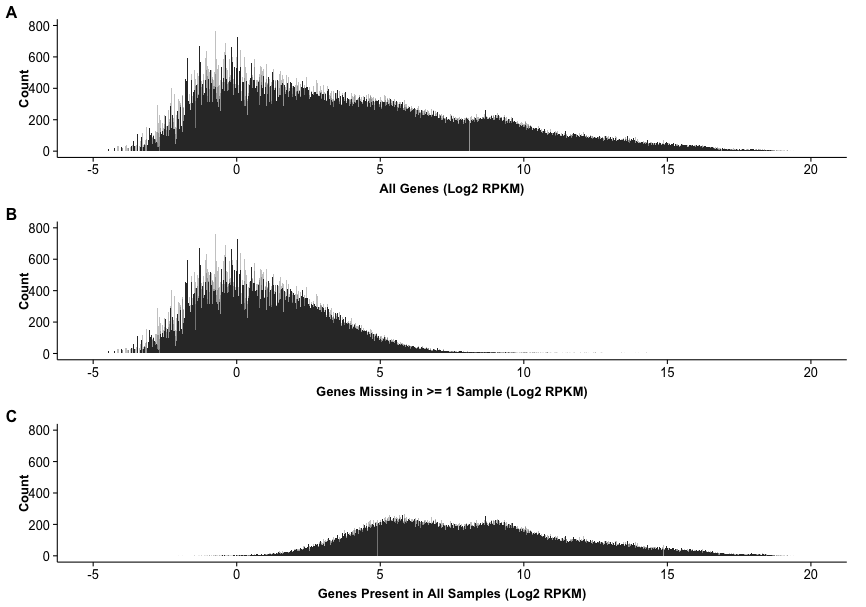
\includegraphics[width=\textwidth]{/Users/eric/Dropbox/thesis/miRNA_Distributions/figure1.png}
  \caption{(A) Histogram of overall microRNA expression in TCGA BRCA microRNA-Seq dataset. 
  (B) Histogram showing expression of microRNAs not expressed
  in at least one sample in TCGA BRCA microRNA-Seq dataset.
  (C) Histogram showing expression of microRNAs present in TCGA BRCA microRNA-Seq dataset.}
\end{figure}

  Histograms of the overall distribution and the full (HE) / partially-missing (LE) gene subsets seem to again support the notion that microRNA expression
can be broken into two distributions based on our chosen criterion. We chose to apply this approach to other cancer types and found that this observation
holds across cancer types from the TCGA data (see Figure \ref{fig::all_tri_plots}). 
We also generated histograms for genes missing in one sample and genes present 
in all samples but have not included the plots in this manuscript. As the 
distributions are so similar, we will show mainly BRCA data as a representation 
of overall trends in the TCGA datasets.

\begin{figure}[H]
 \centering
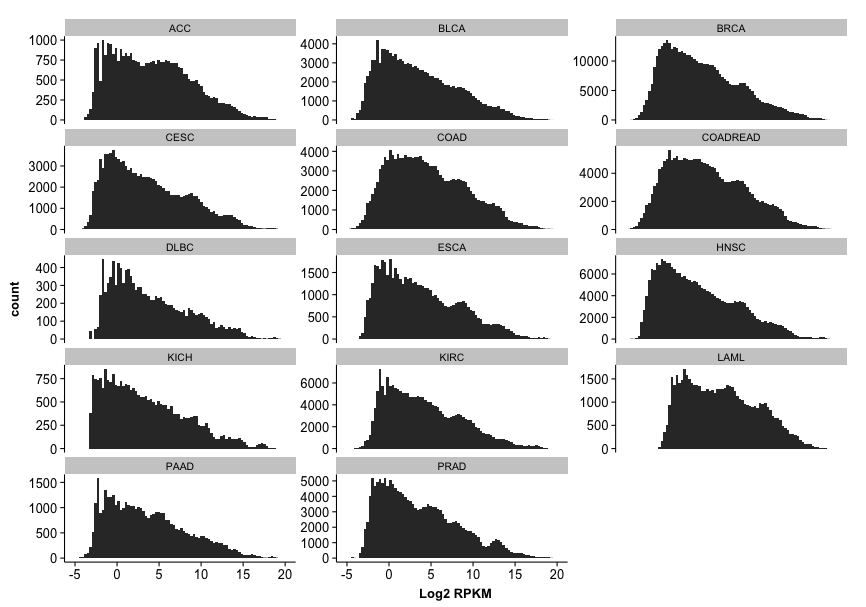
\includegraphics[width=\textwidth]{/Users/eric/Dropbox/thesis/miRNA_Distributions/fig_2_facet_overall.png}
 \caption{Histograms of overall microRNA expression for
 each cancer type from The Cancer Genome Atlas which had an microRNA-Seq dataset.
 Note that y axis values have been scaled for each sample. Overall, the distributions for
 all cancer types look very similar.}
 \label{fig::all_tri_plots}
\end{figure}


%Given that this phenomenon occured in tumor samples we hypothesized that it was also occuring in cells with normal morphology. We examined normal breast cell samples from the
%NCBI Short Read Archive to determine if we saw a similar trend. After aligning the reads and calculating RPKM values, we found that
%NORMAL CELL DATA WOULD GO HERE

  There are several arguments for separating microRNAs based on whether they are present in all samples or not. As we will discuss later, in the samples we analyzed it is extremely rare
  for a microRNA missing in one sample to have an expression level above 5 $\log_{2} \text{RPKM}$. We argue that classifying microRNAs by whether they are missing in any sample or if there expression
  is below 4-5 $\log_{2} \text{RPKM}$ are approximately equivalent approaches. Furthermore, we believe examination of $\log_{2} \text{RPKM}$ data is more informative than raw RPKM levels in the context
  of this study. RPKM is useful for looking at relative expression levels within a sample (). RPKM is also thought to be a decent indicator of RNA abundance, with 1-3 RPKM corresponding to one transcript
  per cell (Mortazavi \textit{et al} 2008), although this notion is hotly contended (see Wagner, Kin, and Lynch 2012). Nonetheless, several studies corroborate that an RPKM value of zero
  means no transcripts for the given RNA are present in the sample (\cite{Hebenstreit2011} ,Mortazavi \textit{et al} 2008, and others). Therefore, microRNAs that are detected in some samples but not
  in others should actually have different transcript counts per cell for the microRNA. We also propose that the microRNAs that are always present in every sample may also represent a core group of essential
  microRNAs and that deletion of one of these is fatal to a cell lineage. As discussed later, this is only one of several possible explanations for this observation, and the experimental work necessary
  to verify this result is outside the scope of this study. %TODO
  
  
  Hebenstreit \emph{et al} used PCR amplification to determine the detection limit of their mRNASeq setup and found that
  genes with values as low as -5 $\log_{2} \text{RPKM}$ could still be detected. These genes mapped to their LE (low-expression) peak. Given this knowledge, we feel comfortable assuming that any microRNA expression that was detected
  was not from experimental noise. As we did not have access to biological samples we could not verify this experimentally.
  
  Of course, the criterion of missing values is exceedingly sensitive to sample size. If sample size is small, chance may dictate whether a given microRNA will be missing from any sample. This disrupts one's ability
  to classify microRNAs. At a sample size of one this ability is completely lost. However, datasets from The Cancer Genome Atlas tend to be large in size ($n > 50$). For BRCA, there are over 1000 samples. Given these
  large sample sizes we believe it is appropriate to continue using this metric. Other methods could also be used, such as a minimum RPKM cutoff or maximum-likelihood determination of distributions. Missing values
  do provide a very useful, convenient method of separating microRNAs into discrete distributions. %TODO
  
  %TODO


\subsection*{KDE Fitting Exposes Substantial Variation in microRNA Expression Distributions}
We next sought to find out how mRNA expression distributions in TCGA data compared to the distributions observed by \cite{Hebenstreit2011} in murine Th2 cells. We first fit kernel density estimates (KDEs) to 
mRNA data to see if the patterns described in the Hebenstreit study were present in cancer data. We generated an overall KDE for the combined mRNA dataset to show
that the overall expression distribution was very similar to that observed in the Hebenstreit study.

%TODO overall KDE for mRNA
\begin{figure}[H]
\centering
 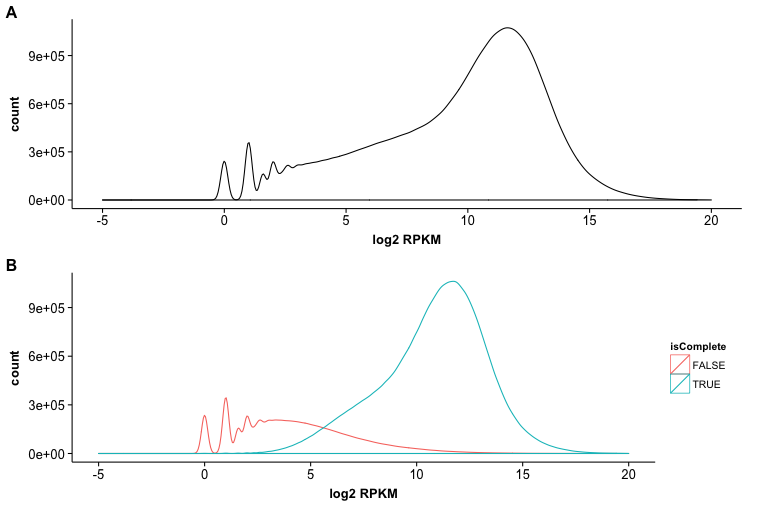
\includegraphics[width=5in]{/Users/eric/Dropbox/thesis/miRNA_Distributions/fig3.png}
 \caption{(A) Kernel density estimate showing the overall expression pattern of microRNAs in the TCGA
 BRCA dataset. (B) Kernel density estimates for microRNAs that are missing in at least one sample (red) or present
 in all samples(blue).}
 \label{fig::brca_mrna_overall_kde}
\end{figure}

We verified that the the majority of mRNAs are expressed at high levels in accordance with the Hebenstreit study.  We present their results here for comparison.

\begin{figure}[H]
\centering
 \includegraphics[width=\textwidth]{/Users/eric/Dropbox/thesis/final_plots/heb_kdes.png}
 \caption{Figure one reprinted from Hebenstreit \textit{et al } 2011.}
 \label{fig::brca_mrna_and_heb}
\end{figure}

We then fit KDEs to individual mRNAs and generated a composite plot of overlayed KDEs. If mRNAs were truly drawn from two distributions, one would expect that these
KDEs would stack over one another, and the underlying distributions could be seen when examining the stacked density estimates. We found that this largely held true for mRNAs.
As can be seen in figure \ref{fig::brca_mrna_kde}, there are major peaks at 0, 1, and 12 $\log_{2} \text{RPKM}$. Hebenstreit \textit{et al} found that major peaks occurred at just above -5 
for ``low-expression'' genes and 5 $\log_{2} \text{RPKM}$ for ``high-expression'' genes. We chose not to pursue exploring this phenomenon, although we believe the shifts in their curves
are from their decision to replace missing $\log_{2} \text{RPKM}$ values with low $\log_{2} \text{RPKM}$ values. We did not to replace missing values in our data, instead opting to remove them
and base summary statistics only on the values present. We believe this more accurately reflects the possible biological ground truth in cancer cells, where gene expression may vary
significantly between samples. There was little support in the literature for either method. %TODO

\begin{figure}[H]
\centering
 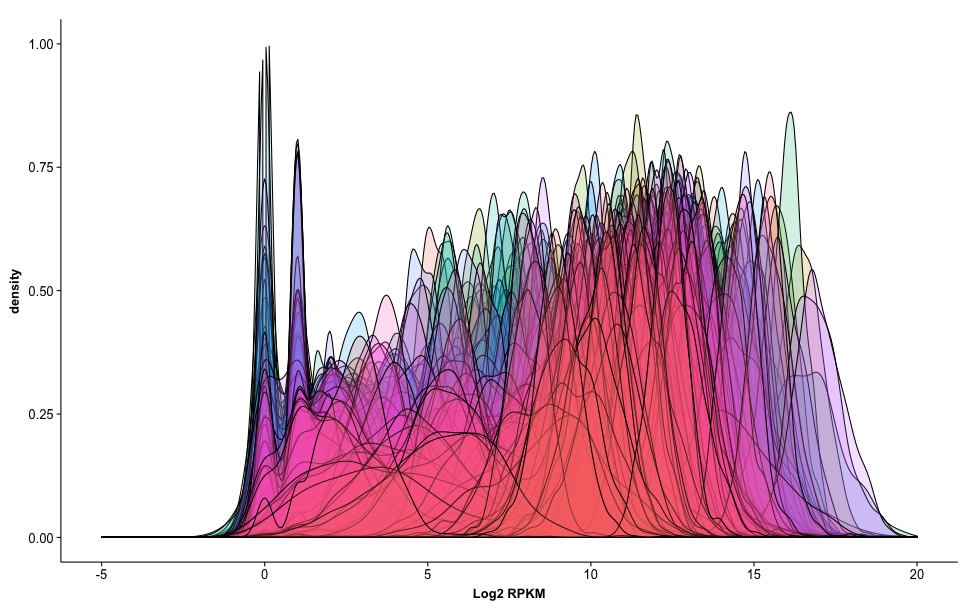
\includegraphics[width=\textwidth]{/Users/eric/Dropbox/thesis/miRNA_Distributions/fig5.png}
 \caption{Composite KDE plot for BRCA mRNASeq data. Each KDE represents the fitted distribution of a single mRNA. There are distinct peaks at 0 and 1 $\log_{2} \text{RPKM}$ and another peak around 12 $\log_{2} \text{RPKM}$.}
 \label{fig::brca_mrna_kde}
\end{figure}



Next we turned to performing the same analysis for microRNAs. We found that microRNAs exhibit an expression distribution pattern that falls in the same range as mRNAs (Figure \ref{fig::brca_mirna_kde}. However,
the relative size of these distributions is opposite those described by Hebenstreit \textit{et al}. The majority of microRNAs are expressed at levels below 5 $\log_{2} \text{RPKM}$ (hereafter LE), while a smaller subset are highly expressed
between 15 and 20 $log_{2} \text{RPKM}$ (HE).

\begin{figure}[H]
\centering
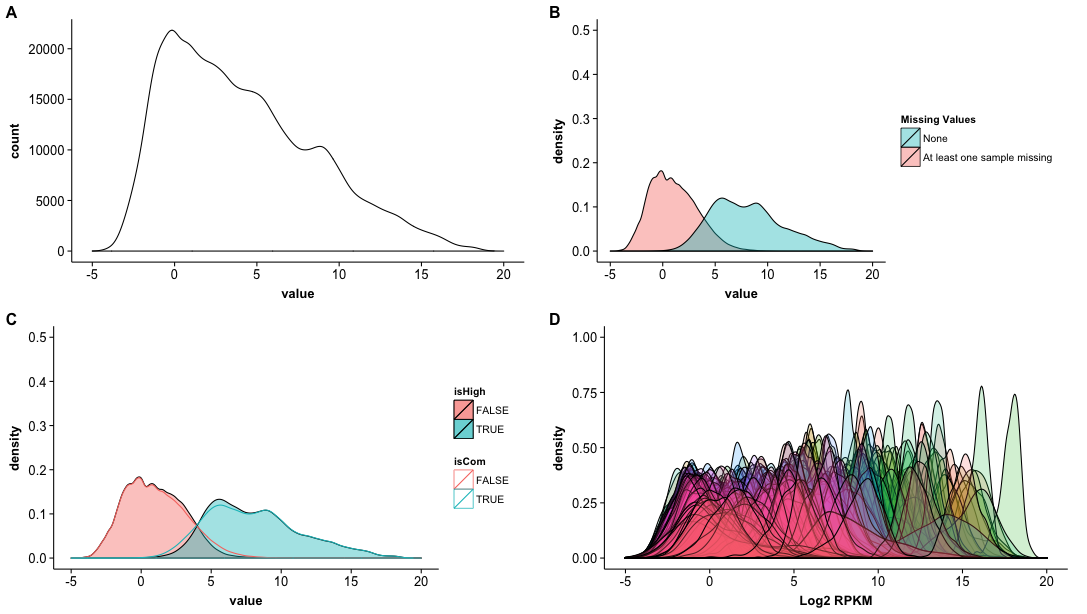
\includegraphics[width=\textwidth]{/Users/eric/Dropbox/thesis/miRNA_Distributions/fig6.png}
\caption{(A) Kernel density estimate of overall distribution of microRNAs in TCGA BRCA dataset.
(B) KDEs showing microRNAs missing in at least one sample or present in all.
(C) Overlaid KDEs for microRNAs missing in some samples or in no samples (fill) 
and those with expression below or above 4 $\log_{2} \text{RPKM} (colored)$.
(D) Overlaid KDEs for all microRNAs in the TCGA BRCA dataset. Peaks are less 
defined than in mRNA data but can still be seen.s
}
 \label{fig::brca_mirna_kde}
\end{figure}
%TODO Pancancer fits of LE/HE/RPKM limits


Close examination of the composite KDE reveals that the two distributions of microRNA expression are less separate than those of mRNAs. While the KDEs do stack around 0 and 7 $log_{2} \text{RPKM}$, many KDEs fall
elsewhere on the range of expression. Figure \ref{fig::brca_mirna_kde}d also shows the equivalency of the missing value criterion and an RPKM cutoff in distinguishing between the two distributions.
%TODO explain this spread

\subsection*{Characterizing MicroRNA Expression Distributions in BRCA}
  We fit normal distributions to the overall, Le, and HE expression groups using the R package MASS. Our results are summarized in figure \ref{fig::fitted_tabular}.
  
  \begin{table}[H]
  \centering
   \caption{Parameter estimates for fitted normal distributions of BRCA microRNA expression using MASS.}
   \begin{tabular}[]{| c | c | c |}
   \hline
    Distribution & Fitted Mean & Fitted SD\\
    \hline 
    Overall& 4.100 & 4.489\\
    \hline
    LE (missing samples present)& 1.053 & 2.228\\
    \hline
    HE (no missing samples) & 8.11373 & 3.441\\
    \hline
   \end{tabular}
  
   \label{fig::fitted_tabular}
  \end{table}

  We then tried pairwaise Kolmogorov-Smirnov (KS) tests to determine whether our fitted distributions were well-fit and whether our two LE and HE distributions were indeed different. All pairwise combinations of KS tests
  indicated that (1) LE and HE microRNAs are drawn from different distributions and (2) fitted distributions were not well-fit to the actual data. Our prediction is that the data is not normally distributed. As negative
  values are possible in log-space, gamma and Weibull are not good options even though their ability to replicate the shape of the distribution would likely be superior.

%TODO write results here; SN analysis.

\subsection*{MicroRNAs With Higher Expression Levels Show Less Variation in Expression}
  We found that microRNAs with average expression levels above roughly 5 $\log_{2} \text{RPKM}$ tend to be expressed in all samples. We first measured variation in expression
  using the mean absolute deviation (MAD), a highly-robust measure of dispersion (). We plotted the MAD for a given gene in the dataset on its median to examine how much variation there was in
  expression as expression levels increased. We colored the data points depending on if the corresponging microRNA was missing in any sample.
  As would be expected the level of variability in expression increases with RPKM. The differences in median RPKM and median absolute deviation in RPKM spanned nearly five orders of magnitude. 
  We then did the same with data that had been $\log_{2}$ transformed
  and found that microRNAs that were expressed at lower levels showed higher fold-change differences. In general, microRNAs that were present in all samples
  tended to show much less variation than did microRNAs which were missing in at least one sample.
  
  \begin{figure}[H]
   \centering
       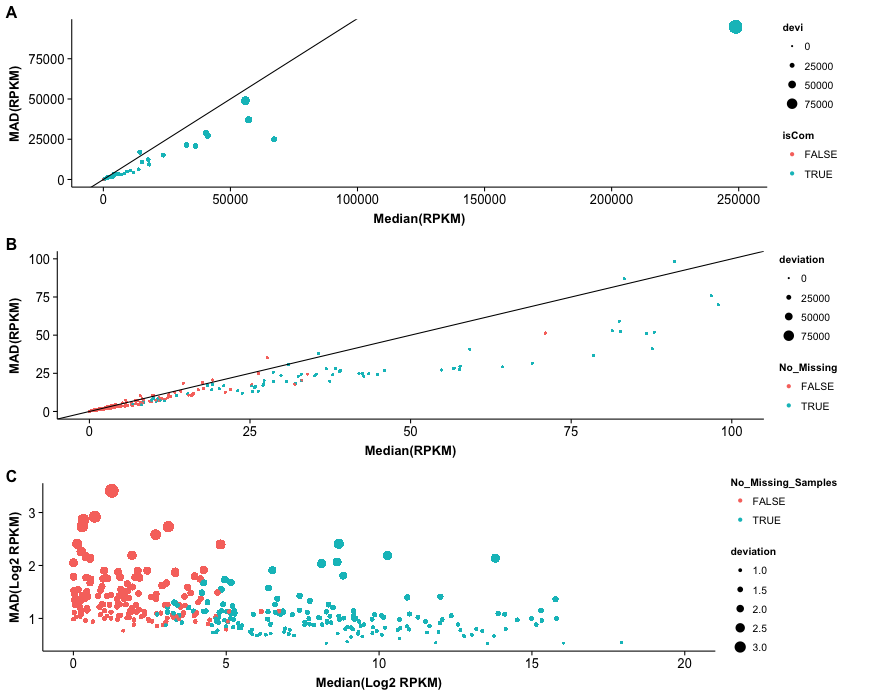
\includegraphics[width=\textwidth]{/Users/eric/Dropbox/thesis/miRNA_Distributions/fig7_a_b_c.png}
        \caption{(A): Overall expression shows median absolute deviation (RPKM) increases directly with median RPKM.
        (B) Plot of median absolute deviation on median expression; scaled to 
        show that microRNAs missing in at least one sample are constrained to 
       much lower RPKM values and lower deviation than those present in all 
       samples.
         (C )Plot of median absolute deviation on median expression after $\log_{2}$ transformation.
         Fold-change variability decreases with increased median expression.}
    \label{fig::mean_on_fig}
  \end{figure}

  There are several possible explanations for why certain microRNAs are never lost in pan-cancer samples. One is that such microRNAs are essential to cell
  survival. Another is that the individual microRNA may be a causative hallmark of the cancer type in which it is detected. MicroRNAs may also tightly follow the
  expression of their targets; any upregulation in a target gene may drive simultaneous upregulation of a targeting microRNA. Testing any of these theories would
  require complex laboratory experiments that are outside the scope of this study.
  
  
\subsection*{Seven $\log_{2}$ RPKM Appears To Be The Lower Bound of Possibly Essential microRNA Expression in TCGA Data}
  We scanned pan-cancer samples to see if we could detect any microRNAs with high average expression (above 4-5 $\log_{2} \text{RPKM}$) that were lost in any samples. We found that 
  above 7 $\log_{2} \text{RPKM}$, it is extremely rare for a microRNA to be deleted. Across all analyzed cancer types, only 0-8 of more than 300 microRNAs were both highly-expressed and missing in at least one sample.
  Refer to figures \ref{fig::all_L_plots} and \ref{fig::all_L_plots_zoom} for pancancer analysis.

  \begin{table}[H]
  \centering
    \caption{MicroRNAs which had median expression levels greater than $\log_{2}(RPKM)$ and were missing in at least one sample for various cancer types.}

  \small
   \begin{tabular}[]{| l | c |}
   \hline
    Cancer Type& microRNA\\
    \hline 
    ACC & \shortstack{
    hsa-mir-377,
    hsa-mir-411,
    hsa-mir-485,\\
    hsa-mir-487a,
    hsa-mir-507,
    hsa-mir-513c,\\
    hsa-mir-655
    }\\
    \hline 
BLCA & \shortstack{hsa-mir-187, hsa-mir-31, hsa-mir-934,\\ hsa-mir-944} \\
\hline 
BRCA & \shortstack{hsa-mir-136, hsa-mir-335, hsa-mir-429,\\ hsa-mir-96}\\
\hline 
COAD & hsa-mir-19a\\
\hline 
COADREAD & hsa-mir-19a\\
\hline 
CESC & \shortstack{hsa-mir-1247, hsa-mir-135b, hsa-mir-944}\\
\hline 
DLBC &\\
ESCA & hsa-mir-944\\
\hline 
HNSC &\shortstack{ hsa-mir-1247, hsa-mir-196a-1, hsa-mir-206}\\
\hline 
KICH & \shortstack{hsa-mir-888, hsa-mir-891b, hsa-mir-892a}\\
\hline 
KIRC & \shortstack{hsa-mir-134, hsa-mir-181c, hsa-mir-193b,\\ hsa-mir-204}\\
\hline 
LAML& \shortstack {hsa-mir-125b-1, hsa-mir-127, hsa-mir-134,\\ hsa-mir-181d, hsa-mir-379, hsa-mir-501,\\ hsa-mir-542, hsa-mir-9-2}\\
\hline 
PAAD & hsa-mir-196b\\
\hline 
PRAD & hsa-mir-205\\
\hline
   \end{tabular}
  \end{table}

We chose to analyze the four microRNAs from this group in BRCA using Ingenuity Target Explorer (QIAGEN, https://targetexplorer.ingenuity.com/). hsa-miR-136 was associated
with HER2 negative breast cancer. hsa-miR-335 regulates cisplatin and paclitaxel and is associated with lung metastasis; it has
roles in differentiation, proliferation, and invasion. hsa-miR-429 is associated with several diverse cancers. Finally,
hsa-miR-96 has a role in development and is associated with colorectal, pancreatic and prostate cancers. We predict there is likely some oncogenic activity from these microRNAs in the
TCGA dataset given these findings.


  
  \begin{figure}[H]
 \centering
 \subfigure[ACC]
 {
 \includegraphics[width=1.75in]{/Users/eric/Dropbox/thesis/final_plots/l_plots/ACC.png}
 }
 \subfigure[BLCA]
 {
  \includegraphics[width=1.75in]{/Users/eric/Dropbox/thesis/final_plots/l_plots/BLCA.png}
 }
 \subfigure[BRCA]
  {
  \includegraphics[width=1.75in]{/Users/eric/Dropbox/thesis/final_plots/l_plots/BRCA.png}
  }
  \\
 \subfigure[CESC]
  {
  \includegraphics[width=1.75in]{/Users/eric/Dropbox/thesis/final_plots/l_plots/CESC.png}
 }
 \subfigure[COAD]
  {
  \includegraphics[width=1.75in]{/Users/eric/Dropbox/thesis/final_plots/l_plots/COAD.png}
 }
 \subfigure[COADREAD]
  {
  \includegraphics[width=1.75in]{/Users/eric/Dropbox/thesis/final_plots/l_plots/COADREAD.png}
 }
 \\
 \subfigure[DLBC]
  {
  \includegraphics[width=1.75in]{/Users/eric/Dropbox/thesis/final_plots/l_plots/DLBC.png}
 }
 \subfigure[ESCA]
  {
  \includegraphics[width=1.75in]{/Users/eric/Dropbox/thesis/final_plots/l_plots/ESCA.png}
 }
 \subfigure[HNSC]
  {
  \includegraphics[width=1.75in]{/Users/eric/Dropbox/thesis/final_plots/l_plots/HNSC.png}
 }
 \\
 \subfigure[KICH]
  {
  \includegraphics[width=1.75in]{/Users/eric/Dropbox/thesis/final_plots/l_plots/KICH.png}
 }
 \subfigure[KIRC]
  {
  \includegraphics[width=1.75in]{/Users/eric/Dropbox/thesis/final_plots/l_plots/KIRC.png}
 }
 \subfigure[LAML]
  {
  \includegraphics[width=1.75in]{/Users/eric/Dropbox/thesis/final_plots/l_plots/LAML.png}
 }
 \\
 \subfigure[PAAD]
  {
  \includegraphics[width=1.75in]{/Users/eric/Dropbox/thesis/final_plots/l_plots/PAAD.png}
 }
 \subfigure[PRAD]
  {
  \includegraphics[width=1.75in]{/Users/eric/Dropbox/thesis/final_plots/l_plots/PRAD.png}
 }
 \caption{Plots showing the number of samples missing a microRNA as related to the median $\log_{2} \text{RPKM}$. In general, microRNAs that are highly expressed appear in almost every sample.}
 \label{fig::all_L_plots}
\end{figure}
  
  
  \begin{figure}[H]
 \centering
 \subfigure[ACC]
 {
 \includegraphics[width=1.75in]{/Users/eric/Dropbox/thesis/final_plots/l_plots/ACC_zoom.png}
 }
 \subfigure[BLCA]
 {
  \includegraphics[width=1.75in]{/Users/eric/Dropbox/thesis/final_plots/l_plots/BLCA_zoom.png}
 }
 \subfigure[BRCA]
  {
  \includegraphics[width=1.75in]{/Users/eric/Dropbox/thesis/final_plots/l_plots/BRCA_zoom.png}
  }
  \\
 \subfigure[CESC]
  {
  \includegraphics[width=1.75in]{/Users/eric/Dropbox/thesis/final_plots/l_plots/CESC_zoom.png}
 }
 \subfigure[COAD]
  {
  \includegraphics[width=1.75in]{/Users/eric/Dropbox/thesis/final_plots/l_plots/COAD_zoom.png}
 }
 \subfigure[COADREAD]
  {
  \includegraphics[width=1.75in]{/Users/eric/Dropbox/thesis/final_plots/l_plots/COADREAD_zoom.png}
 }
 \\
 \subfigure[DLBC]
  {
  \includegraphics[width=1.75in]{/Users/eric/Dropbox/thesis/final_plots/l_plots/DLBC_zoom.png}
 }
 \subfigure[ESCA]
  {
  \includegraphics[width=1.75in]{/Users/eric/Dropbox/thesis/final_plots/l_plots/ESCA_zoom.png}
 }
 \subfigure[HNSC]
  {
  \includegraphics[width=1.75in]{/Users/eric/Dropbox/thesis/final_plots/l_plots/HNSC_zoom.png}
 }
 \\
 \subfigure[KICH]
  {
  \includegraphics[width=1.75in]{/Users/eric/Dropbox/thesis/final_plots/l_plots/KICH_zoom.png}
 }
 \subfigure[KIRC]
  {
  \includegraphics[width=1.75in]{/Users/eric/Dropbox/thesis/final_plots/l_plots/KIRC_zoom.png}
 }
 \subfigure[LAML]
  {
  \includegraphics[width=1.75in]{/Users/eric/Dropbox/thesis/final_plots/l_plots/LAML_zoom.png}
 }
 \\
 \subfigure[PAAD]
  {
  \includegraphics[width=1.75in]{/Users/eric/Dropbox/thesis/final_plots/l_plots/PAAD_zoom.png}
 }
 \subfigure[PRAD]
  {
  \includegraphics[width=1.75in]{/Users/eric/Dropbox/thesis/final_plots/l_plots/PRAD_zoom.png}
 }
 \caption{Plots showing the number of samples missing a microRNA as related to the median $\log_{2} \text{RPKM}$, scaled to show only the microRNAs missing in fewer than ten samples.
 In general, microRNAs that are highly expressed appear in almost every sample.}
 \label{fig::all_L_plots_zoom}
\end{figure}  
  
\subsection*{Tumors Differ More in Highly-Expressed Than Lowly-Expressed microRNAs}

To assess if one distribution of microRNAs might be more useful in clustering tumor samples we performed a series of unsupervised hierarchical clusterings. We clustered
tumors by their overall microRNA expression, the expression of their LE genes, and the expression of their HE genes as defined by the missing sample criterion (figure \ref{fig::dendros}).

\begin{figure}[H]
  \centering
  \subfigure[]{
   \includegraphics[width=3.5in]{/Users/eric/Dropbox/thesis/final_plots/dendros/dendro_all.png}
  }
  \subfigure[]{
   \includegraphics[width=3.5in]{/Users/eric/Dropbox/thesis/final_plots/dendros/dendro_le.png}
  }
  \subfigure[]{
   \includegraphics[width=3.5in]{/Users/eric/Dropbox/thesis/final_plots/dendros/dendro_HE.png}
  }
  \caption{Pancancer dendrograms of microRNA expression distributions.
  (A) Hierarchical clustering dendrogram for overall microRNA expression.
  (B) Hierarchical clustering dendrogram for LE microRNA expression
  (C) Hierarchical clustering dendrogram for HE microRNA expression}
 \label{fig::dendros}
\end{figure}

This analysis clearly showed that HE microRNA expression provided the cleanest clustering result. LE genes showed very little separation among samples; this may have been because each
cancer type had too many in common or expression within each cancer type may have been too divergent to distinguish cancer of one type from another. It is known that clustering of cancer
samples by a variety of methods tends to recover the cell type of the tissue of origin \cite{Gaur2007}. This information is often of negligible use in the clinic.

%TODO Finish describing this. Try to analyze why HE gives better separation. Try to get even better separation.s

%\subsection*{GO Analysis}

%\subsection*{Comparing Normal and Tumor miRNA Expression}


\section*{Discussion}
  This analysis demonstrated that microRNA expression in data from The Cancer Genome Atlas can be
  characterized by two overlapping distributions. These distributions have similar characteristics but
  different frequencies compared to those described by Hebenstreit \emph{et al} in their 2011 study of
  murine Th2 cells \cite{Hebenstreit2011}. One distribution (termed LE) contains microRNAs that are occasionally deleted in samples 
  while the other (HE) contains microRNAs that are never deleted in our dataset. HE microRNAs tend to have significantly higher median
  expression than LE ones. in BRCA, LE microRNAs tend to be expressed below about 4 $\log_{2} \text{RPKM}$ 
  while HE microRNAs are generally expressed above this threshold. The presence of two distributions holds across
  all cancer types in our analysis. We find that microRNAs with 
  median expression above about 7 $\log_{2} \text{RPKM}$ are not deleted in any 
  of the nearly 5,000 samples in our dataset. In general, there is a strong 
 correlation between a microRNA's median expression in $\log_{2} \text{RPKM}$ and the 
 number of samples missing that microRNA ($-.592, p << .001$ in BRCA). We also 
 observed that while HE microRNAs tend to have higher absolute changes in 
 expression as measured by raw RPKM, LE microRNAs show higher fold-change variability.
 Finally, we examined the clustering abilities of each distribution using 
 agglomerative hierarchical clustering. Tumors from different cancer types showed much more heterogeneity in 
 their overall and HE microRNAs than in their LE microRNAs. All of the trends we 
 discuss hold across all of the cancer types in our analysis.
  
  We also replicated the kernel density estimates of \cite{Hebenstreit2011} for messenger RNA 
  data. We found that the
  magnitude of our results differed greatly, with our data showing globally higher expression.
   We are unsure whether this
  phenomenon is relevant to the cancer phenotype or if it is an artifact of
  experimental protocol. Considering the reservations of
  many scientists with regards to RNA-Seq interpretation \cite{Wagner2012} we are not confident
  we could answer this question without obtaining raw data from The Cancer Genome Atlas.
  
  Our choice to use the presence of missing samples as a criterion for 
  separating distributions is supported by the idea that this distribution is a 
  subset of lowly-expressed genes. While a superior method would be to classify 
  microRNAs into LE or HE distributions using a machine learning approach, we 
  leave this analysis to another group. Such an approach, while useful, would 
  undoubtedly be difficult to verify without access to experimental data. If we 
  assume as Hebenstreit \emph{et al} do that there exist a set of essential 
  genes in our analysis, it is within reason to also assume that microRNAs deleted in 
  even a single sample are not essential to cell survival. This gives us a very 
  simple criterion for separating our microRNAs based on their biological 
  necessity. Conveniently, this method also aligns well with distinct expression 
  levels. We expect that classification of microRNAs by machine learning would 
  reveal that our missing-sample criterion constitutes a subset of true 
  lowly-expressed microRNAs.
    
  Interestingly, there appears to be a 
  relatively firm upper bound above which it is exceedingly rare to see deletion 
  of a microRNA. There are several possible explanations for this. It is 
  possible that the log-fold changes in expression even at low $\log_{2} \text{RPKM}$ 
  may be sufficient to alter the expression of a microRNA's targets. There is some support for this
  notion in the literature. In general, microRNAs with many targets do in fact shower greater cellular effects
  when their fold-change expression is altered \cite{Calin2006, Lim2005}. It is 
  interesting then that fold-change differences are greater in the LE 
  distribution of microRNAs, as these appear to be non-essential microRNAs based 
  upon our missing-sample criterion. An alternative explanation is that 
  highly-expressed microRNAs are amplified in cancer cells. Indeed, HE microRNAs are associated with 
  many important cellular processes based on preliminary functional analysis results of a subsample of HE microRNAS using QIAGEN’s Ingenuity Target Explorer. It seems plausible then that 
  HE microRNAs are essential to the cell. It is perhaps possible, therefore, 
  that smaller changes in log-fold expression are sufficient to affect their 
  targets. We believe this second explanation to be better than the first, 
  though without experimental data we have no way of truly verifying our 
  suspicions. There is also notable bias in microRNA functional analysis 
  \cite{Bleazard2015}. We expect that future experiments will verify that 
  microRNAs in the HE distribution are important, though perhaps less essential 
  than ITE results indicate.
  
  The differing ability of the LE and HE distributions to cluster tumor samples 
  is perhaps the most poignant result of this study as it has the most direct 
  application to the multi-omics models of interest in the field. In multi-omics 
  models, each biological factor examined constitutes another variable under analysis. If 
  LE genes are not important to clustering but are included in a given model 
  then that model has been over-parameterized. It is admittedly possible that 
  the HE distribution contains cell type marker microRNAs. If this is the case 
  we would expect tumors of the same cancer type to cluster together more when 
  HE genes are examined than when clustering is performed using the entire 
  microRNA transcriptome. There is not strong evidence of this happening in our 
  analysis. If experimental results corroborate the ability of HE microRNAs to 
  differentiate tumors by molecular pathology then we propose that multi-omics 
  models should only consider HE microRNAs in their analysis.
  
  Given the poor results of normal distributions fit to the data, we expect a 
  different distribution would be more appropriate. Unsupervised clustering
  of microRNAs based on expression level might help in informing 
  which model should be fit. We expect that a skew-normal distribution would 
  have fit better but avoided the additional complexity of attempting to fit 
  one. Gamma, beta or Weibull might also be appropriate if their distributions 
  are shifted to accommodate negative values in the $\log_{2} \text{RPKM}$ data.
  It cannot be ruled out that more than two distributions exist in expression data. 
  We leave it to someone with sufficient knowledge of statistical classification 
  to prove how many distributions are appropriate.
  
  
 Our results provide support for the presence of two distributions in 
 microRNA-Seq data from cancer cells. Preliminary results from normal cell data 
 indicate that two distributions may also exist in normal human cell microRNA 
 expression. However, access to normal human data is extremely limited due to 
 privacy concerns. Other groups have compared the expression differences of 
 individual microRNAs in tumor and normal cells but no examination of the 
 overall distributions has been done to our knowledge. We believe such an 
 analysis could help generate a somatic microRNA expression difference profile 
 that might be useful in multi-omics models. In addition, integrating mutations 
 in microRNA sequence would be useful for a variety of reasons. As microRNAs use 
 Watson-Crick base pairing in only a small seed region to modulate expression of their targets \cite{Bartel2009}, sequence 
 mutations may have a significant effect on downstream gene expression without 
 affecting microRNA-Seq results. Our hope and our suspicions are that the 
 results presented herein only scratch the surface of what may prove to be very 
 valuable knowledge to developers of multi-omics models.
  
  
  

\bibliography{thesis_biblio}
\bibliographystyle{plain}


\end{document}
